\documentclass[a4paper,12pt]{article}
\usepackage[margin=1in]{geometry}

\usepackage[T2A]{fontenc}			% кодировка
\usepackage[utf8]{inputenc}			% кодировка исходного текста
\usepackage[english,russian]{babel}	% локализация и переносы
\usepackage{graphicx}                % Математика
\usepackage{amsmath,amsfonts,amssymb,amsthm,mathtools} 
\usepackage{mathtext}
\usepackage[T2A]{fontenc}
\usepackage[utf8]{inputenc}

\usepackage{wasysym}

%Заговолок
\author{Бичина Марина 
группа Б04-005 1 курса ФЭФМ}
\title{}
\date{}


\begin{document} % начало документа

\begin{center}
\begin{Large}
{ Марина Б04-005, Лабораторная работа №.3.1.3 Измерение магнитного поля Земли}
\end{Large}
\end{center}
\paragraph{Цель работы:} 
\begin{enumerate}
\itemsep0em
\item Исследовать свойства постоянных неодимовых магнитов
\item Измерить с их помощью горизонтальную и вертикальную составляющие индукции магнитного поля Земли и магнитное наклонение 
\end{enumerate}
\paragraph{Оборудование:}
\begin{enumerate}
\itemsep0em
\item 12 одинаковых неодимовых магнитов
\item тонкая нить для изготовления крутильного маятника
\item медная проволока
\item электронные весы
\item секундомер
\item измеритель магнитной индукции
\item штангенциркуль
\item бруски
\item линейка и штатив из немагнитных материалов
\item набор гирь и разновесов
\end{enumerate}


\paragraph{Теоретическая справка:}
\paragraph{}
Магнитный момент $\overrightarrow{m}$ диполя, которыми являются неодимовые шарики в данной работе, можно вычислить по формуле 
\begin{equation}
\overrightarrow{m} = \frac{1}{c}I\cdot S \cdot \overrightarrow{n} 
\end{equation}
где I - ток, протекающий в витке, площади S, направленный по нормали к площади.\\
Поле магнитного диполя совпадает с формулой для электрического диполя:
\begin{equation}
B_{d} = \frac{3(\overrightarrow{m},\overrightarrow{r})\overrightarrow{r}}{r^5} -\frac{\overrightarrow{m}}{r^3}
\end{equation}
Силу взаимодействия двух одинаковых магнитов можно рассчитать по формуле
\begin{equation}
F_{12} = \overrightarrow{m_1}\frac{dB_2}{dr} = -6\frac{\overrightarrow{m_1} \overrightarrow{m_2}}{r^4} = -6\frac{\overrightarrow{m_1}^2}{r^4}
\end{equation}
Для метода B мы рассматриваем силу, равную
\begin{equation}
F=F_0(1+\frac{1}{2^4}+\frac{1}{3^4}+\frac{1}{4^4})\approx 1.08F_0
\end{equation}
Период крутильных колебаний маятника
\begin{equation}
T_{n}=2\pi sqrt{\frac{mR^2}{3\overrightarrow{m}B_{\parallel}}}\cdot n
\end{equation}
Момент силы тяжести
\begin{equation}
\textbf{\emph{M}} = n\overrightarrow{m}B_{\perp}
\end{equation}
\paragraph{}

\paragraph{Описание установки:}
\paragraph{Пункт 1: Определение магнитного момента магнитных шариков}
\begin{enumerate}
\itemsep0em
\item \textbf{Метод А}
Величину магнитного момента $\overrightarrow{m}$ можно узнать, определив максимальное расстояние между двумя одинаковыми шариками, на котором они еще удерживают друг друга в поле тяжести. При максимальном расстоянии сила тяжести шариков равна силе их магнитного притяжения. Тогда по формуле (3) мы можем определить магнитный момент шариков. По формуле (2) можно найти индукцию поля.
\begin{figure}[h!]
\centering
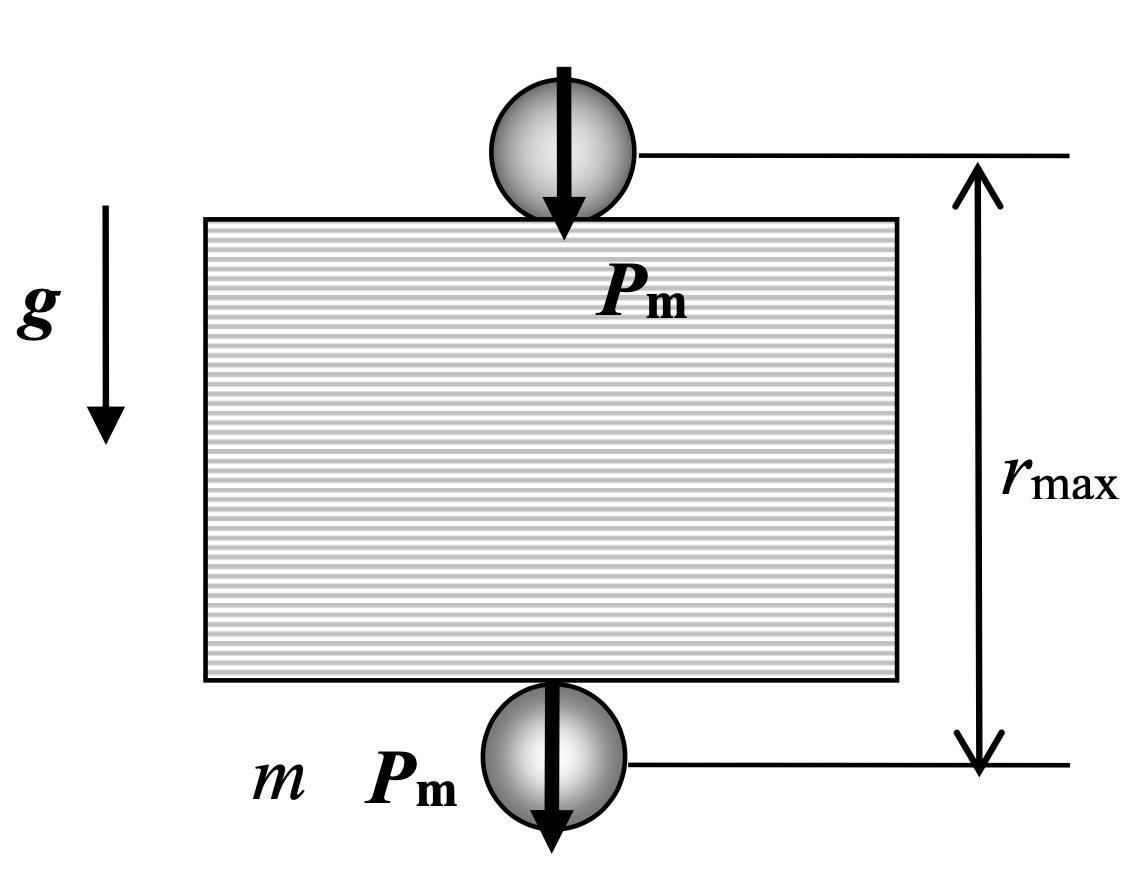
\includegraphics[scale=0.25]{ris1.png} 
\caption{измерение магнитных моментов шариков}
\end{figure} \\
\item \textbf{Метод Б} заключается в поиске силы сцепления шариков (т.е. силы, необходимой для разрыва двух сцепившихся магнитных шариков). Ее можно определить по весу магнитной цепочки, которую способен удержать самый верхний магнитный шарик. При расчетах мы будет использовать приближение (4)
\begin{figure}[h!]
\centering
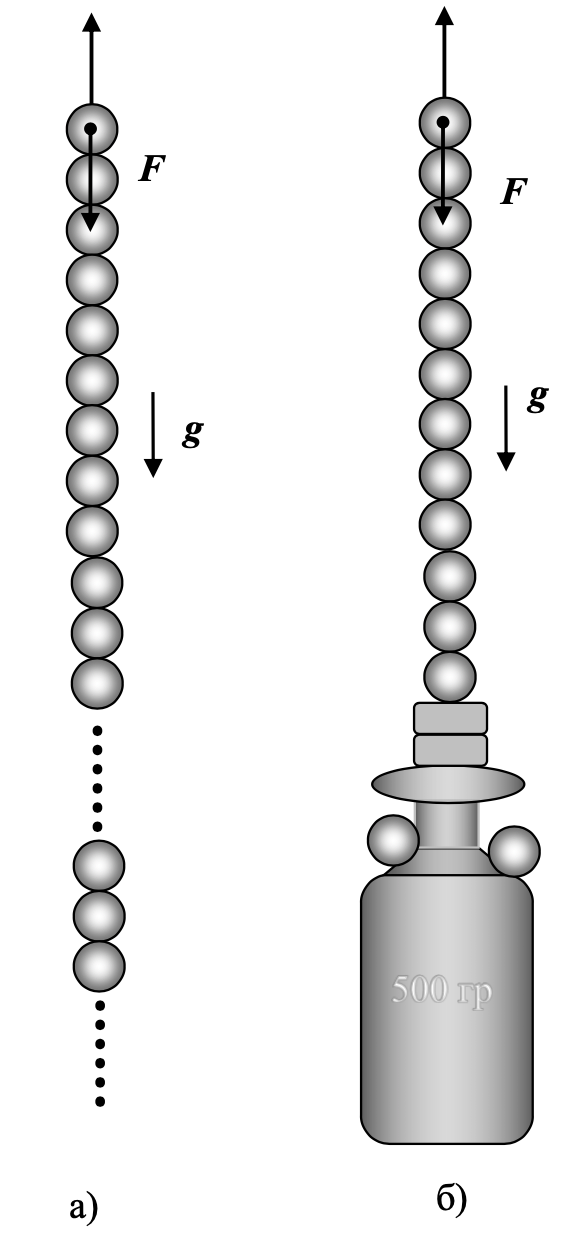
\includegraphics[scale=0.25]{ris2.png}
\caption{альтернативный способ измерения магнитных моментов шариков} 
\end{figure}
\end{enumerate}
\paragraph{Пункт 2: Измерение горизонтальной составляющей индукции магнитного поля Земли}
Магнитное поле можно определить по периоду крутильных колебаний "магнитной стрелки", образованной сцепленными друг с другом намагниченными шариками, закрепленными на нитке. Рассчитать это можно по формуле (5). 
\begin{figure}[h!]
\centering
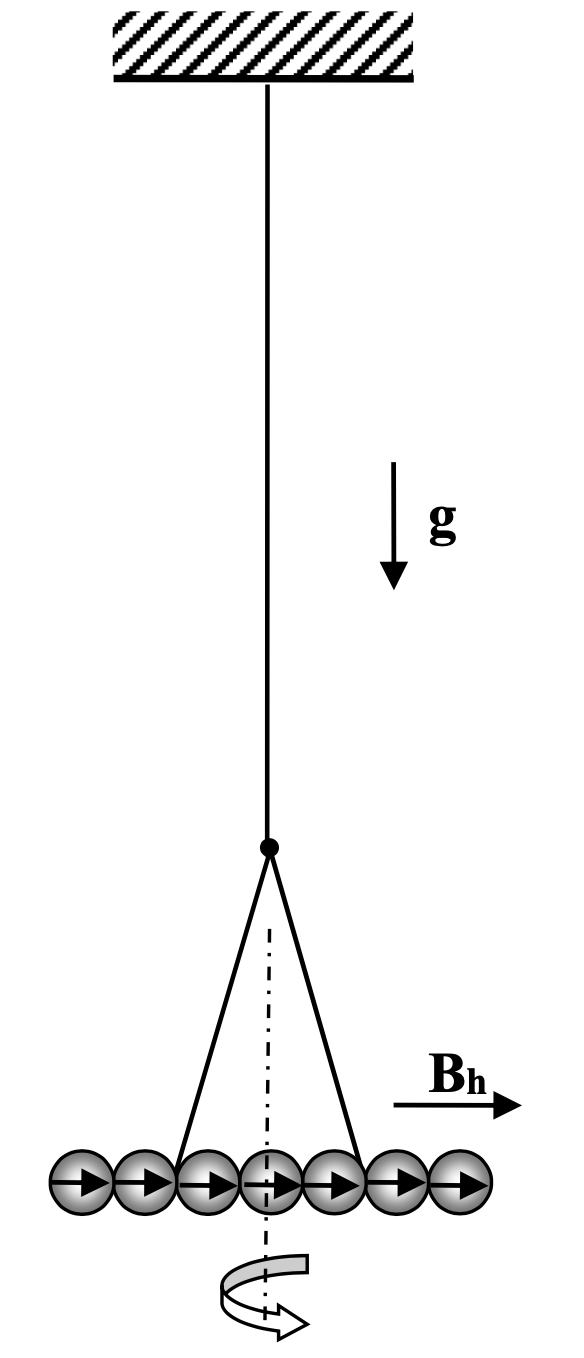
\includegraphics[scale=0.25]{ris3.png} 
\caption{крутильный маятник во внешнем магнитном поле}
\end{figure}
\paragraph{Пункт 3: Измерение вертикальной составляющей индукции магнитного поля Земли. Магнитное наклонение.}
Установка для измерения вертикальной составляющей похожа на установку для п2, только нить будет привязана к центру "магнитной стрелки". Для рассчета мы будет использовать формулу (6). 
\begin{figure}[h!]
\centering
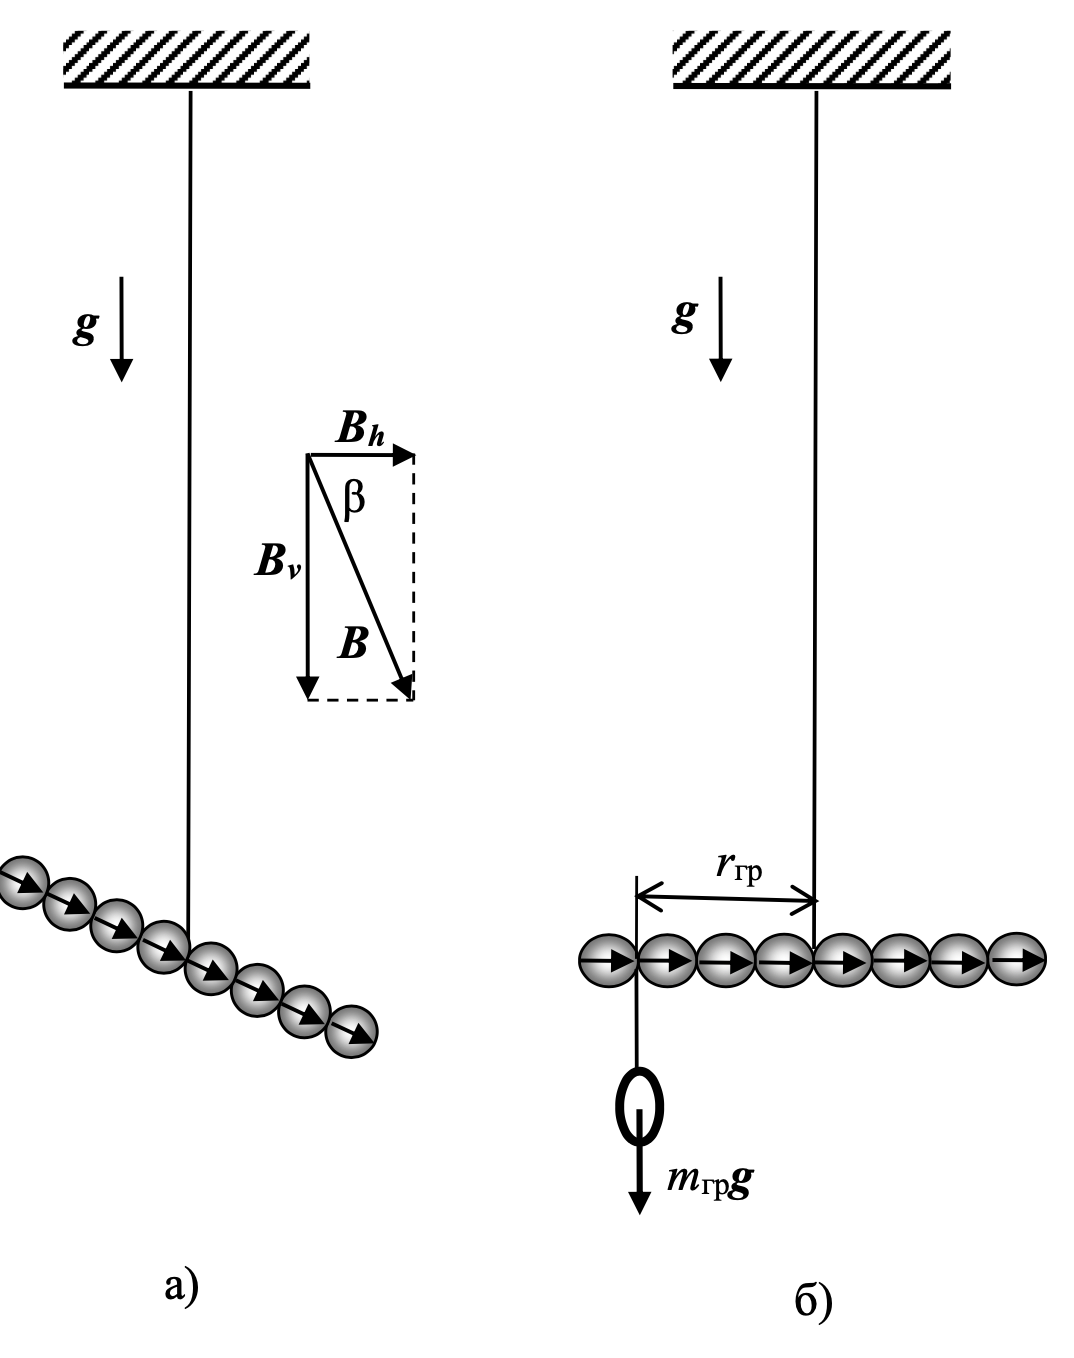
\includegraphics[scale=0.25]{ris4.png} 
\caption{измерение вертикальной составляющей поля магнитного наклонения}
\end{figure}
\paragraph{Ход работы:}
\begin{enumerate}
\itemsep0em
\item Взвесим шарики на весах. Можно считать, что магнитное взаимодействие с весами несущественны для измерения веса. $m_0\cdot N = 8.234 \;\; =>\;\; m_0 = 0.8234\approx 0.82$ г
\item П1 метод А: получим $d\approx 20.6$ мм - расстояние между шариками. По 2 закону Ньютона + формуле (3) рассчитаем $\overrightarrow{m} = \sqrt{\frac{mgr^4}{6}} = 49,2\;$ эрг/Гс\\
За погрешность примем толщину деревянной линейки: $\sigma_{r}\approx 2\;$ мм, тогда $\sigma_{m} = 6.8$ эрг/Гс\\
Рассчитаем индукцию магнитного поля: $B_{m} \approx 283 \;$ мТл, $\sigma_{B} = 40$ мТл\\
Окончательно: $B_{m} = 280\pm 40$ мТл
\item П1 метод Б: Максимальный груз, который выдерживает верхний шарик равен $m_{max}=322.94$ г \\
Сила сцепления тогда равна:\\
$F_0=\dfrac{F}{1.08}=\dfrac{m\cdot g}{1.08}\approx 293 \cdot 10^3$ дин \\
$F_0 = \dfrac{6\cdot \overrightarrow{m}^2}{r^4} => \overrightarrow{m}=r^2\cdot\dfrac{F_0}{6}\approx 94.235$ эрг/Гс\\
Погрешность равна:\\
$\sigma_{m}=8.33$ эрг/Гс\\
$B_{m}=\dfrac{2\cdot \overrightarrow{m}}{r^3}\approx 5415.22$ эрг/$\text{Гс}\cdot \text{см}^3$\\
Окончательно $B_m = 541.5 \pm 48.7$ мТл
\item П2: Исследуем зависимость периода крутильных колебаний стрелки $T$ от количества шариков $n$:\\
Сперва убедимся,что модуль кручения нитки не сильно влияет на конечный результат. Свернем магнитную стрелку в кольцо. Увидим, что период становится больше более чем в 2 раза, из этого можно сделать, что модулем кручения действительно можно пренебречь.
\begin{table}[h!]
\centering
\begin{tabular}{|l|l|l|l|l|l|l|l|}
\hline
n   & 12    & 12    & 12    & 10    & 10    & 8     &       \\ \hline
Т,с & 3,11  & 3,147 & 3,125 & 2,604 & 2,628 & 2,044 &       \\ \hline
n   & 8     & 6     & 6     & 4     & 4     & 2     & 2     \\ \hline
T,c & 2,119 & 1,407 & 1,417 & 0,941 & 0,935 & 0,675 & 0,682 \\ \hline
\end{tabular}
\end{table}
Построим график зависимости $T(n)$ \\
Угловой коэффициент для нашей прямой будет равен:
\\
$
l = 0.257 \; \text{с},
$
$
\sigma_{l} = \dfrac{1}{\sqrt{N}}\sqrt{\dfrac{\langle T^2 \rangle - \langle T \rangle ^ 2}{\langle n^2 \rangle - \langle n \rangle ^ 2} - k^2} = 0.007 \; \text{с}.
$

\begin{figure}[h!]
\begin{center}
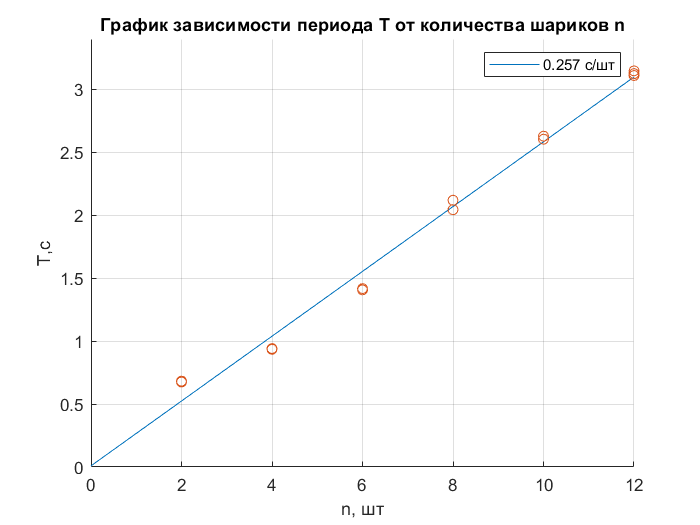
\includegraphics[scale=0.6]{plot1.png} 
\caption{Первый график}
\label{plot1}
\end{center}
\end{figure}

Выражаем коэффициент наклона из формулы:
$ k = 2 \pi \sqrt{\dfrac{m R^2}{3 P_m B_\parallel}} = 2\pi \sqrt{\dfrac{m}{B_r R B_\parallel}} \Rightarrow B_\parallel = \dfrac{4 \pi^2 m}{k^2 B_r R}.
$\\
Подставим полученные и табличные значения в формулу:

$ B_\parallel = 0.139 \;\; \text{мТл}$
\\
$\sigma_B  = 0.01 \;\;\text{мТл}.
$

Получаем $B_\parallel = 0.139 \pm 0.01$ мТл.
\item П3: Для различных значений $n$ уравновесим стрелку, и измерим приложенный момент сил $M_n$ при помощи весов дли измерения массы груза $m_n$ и известного диаметра шара для измерения плеча силы $r_n$ ($M_n = m_n g r_n$).
\begin{table}[h!]
\centering
\begin{tabular}{|l|l|l|l|l|l|}
\hline
n         & 4   & 6   & 8   & 10  & 12  \\ \hline
M, дин*см & 121 & 204 & 204 & 306 & 518 \\ \hline
\end{tabular}
\end{table}
Построим график зависимости $M(n)$
\begin{figure}[h!]
\begin{center}
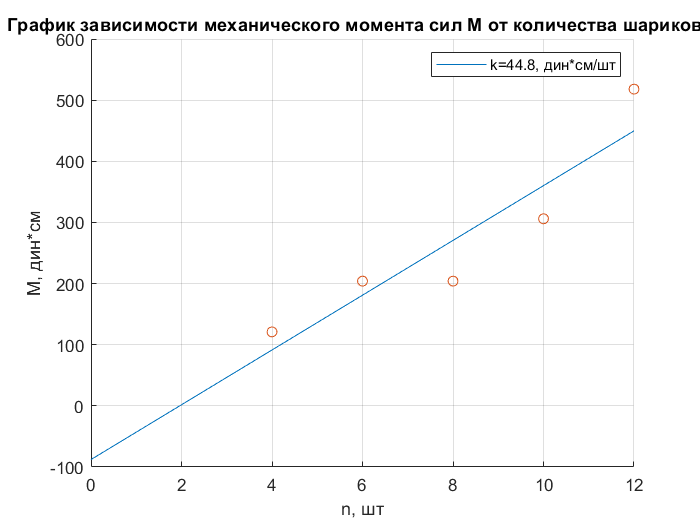
\includegraphics[scale=0.6]{plot2.png}
\caption{Второй график}
\label{plot2}
\end{center}
\end{figure}

Выразим коэффициент наклона из формулы (6):

$ B_\perp = 0.04 \text{мТл}
$

$ \sigma_\alpha = 0.008 \; \text{мТл}.
$

Получаем $B_\perp = 0.040 \pm 0.008$ мТл.
\item Рассчитаем магнитное наклонение и полную индукцию магнитного поля Земли 

Полная индукция магнитного поля Земли равна $B = \sqrt{B_\parallel^2 + B_\perp^2} = \sqrt{0.139^2 + 0.04^2} = 0.144$ мТл. Погрешность $\sigma_B = \sqrt{\sigma_{B \parallel}^2 + \sigma_{B \perp}} = \sqrt{0.09^2 + 0.08^2} = 0.012$ мТл. Получаем значение $B = 0.139 \pm 0.012$ мТл.
\\ Вычислим магнитное наклонение $\beta$:

$\beta =\arctan{\dfrac{B_{\perp}}{B_{\parallel}}} = 33^o
$

\end{enumerate}
\paragraph{Выводы:}
\begin{enumerate}
\item Мы определили магнитный момент магнитных шариков 2 различными способами. Методом А получили результат, равный $\overrightarrow{m}=49.2\;\;\frac{\text{эрг}}{\text{Гс}}$, методом Б - $\overrightarrow{m}=94.235\;\;\frac{\text{эрг}}{\text{Гс}}$. Такая большая разница может возникнуть из-за того, что мы неточно измерили расстояние в методе А, а в методе Б не учли взаимодействие других магнитов (мы рассмотрели взаимодействие только верхнего магнита с 3 ближайшими соседями.
\item Исследовали период крутильных колебаний стрелка T от числа шариков. Заметим, что график начинается в 0, что соответствует теории. Получили параллельную составляющую магнитного поля Земли $B_{\parallel}=0.139 \pm 0.01\;\;\text{мТл}$
\item Рассмотрели зависимость момента силы тяжести от числа шариков. Получили, что график начинается не с 0, а с -87 дин*см, что говорит о неточности наших измерений. Далее получили перпендикулярную составляющую $B_{\perp}=0.04 \pm 0.008\;\;\text{мТл}$
\item Нашли индукцию магнитного поля Земли,$B=0.139 \pm 0.012\;\;\text{мТл}$
\item Нашли магнитное наклонение $\beta = 33^o$ что расходится с табличным $\beta = 61^o$
\end{enumerate}
\end{document}